%label:"art:tropicalGeometryIntersectionIntroduction"
%type:"article"
%name:"a sketch of intersection theory"
%parent:"art_tropicalGeometrySeminarOutline"



Given $Z_k(\RR^n)$, the set of tropical $k$-cycles, has a group structure, whose additive structure is given by taking unions and subdividing. This also comes with a ring structure 
\begin{align*}
    Z_k(\RR^n)\otimes Z_l(\RR^n)\to \ZZ_{n+l-n}(\RR^n)\\
    X\tensor Y \mapsto \lim_{\epsilon\to 0} (X\cap (T+\eps v))
\end{align*}
where is chose so that the intersection is transverse for all $\epsilon>0$ sufficiently small. 

%label:"fig:intersectionoftropicalcurves"
%author:JeffHicks
%name:"intersection of tropical curves"
%type:"figure"
%parent:"art_tropicalGeometryIntersection"
%caption:"We compute the intersection between the two tropical curves drawn on the left hand side by first taking a slight perturbation so that they intersect transversely. The set obtain in the limit as the perturbations go to zero is independent of the choice of transverse perturbation. In this setting, the intersection of two tropical lines is a point."
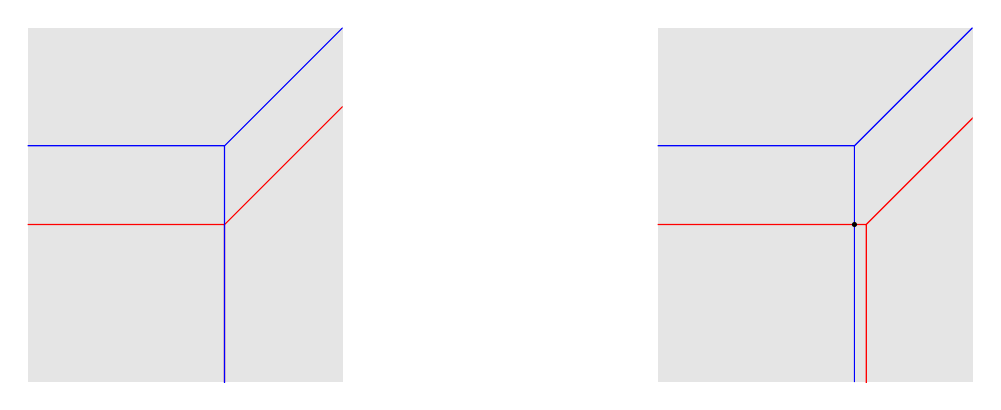
\begin{tikzpicture}\begin{scope}[shift={(0,0)}]

        \fill[gray!20]  (1.5,2) rectangle (-2.5,-2.5);
        \clip  (1.5,2) rectangle (-2.5,-2.5);
                \draw[blue] (-2.65,0.5) -- (0,0.5) -- (0,-2.5) (1.5,2) -- (0,0.5);
                \draw[red] (-3,-0.5) -- (0.15,-0.5) -- (0.15,-3) (1.65,1) -- (0.15,-0.5);
                
        \node[circle, fill=black, scale=.2] at (0,-0.5) {};
        \end{scope}
        
                    \begin{scope}[shift={(-9,1)}]
                    \fill[gray!20]  (2.5,1) rectangle (-1.5,-3.5);
                    \clip  (2.5,1) rectangle (-1.5,-3.5);
        \draw[red] (-2,-1.5) -- (1,-1.5) -- (1,-3.5) (2.5,0) -- (1,-1.5);
                    \draw[blue] (-2.5,-0.5) -- (1,-0.5) -- (1.0001,-4) (2.5,1) -- (1,-0.5);
        
        \end{scope}
                \end{tikzpicture}
        

The key step to proving that this ring structure is well defined is the moving lemma. 
%label:"lem:movinglemma"
%type:"lemma"
%name:"moving lemma"


    The content of the moving lemma goes here


From this information, it is natural to define a tropical version of the Chow group. This means that we need a substitute for rational/algebraic/numerical equivalence. 
%label:"def:TropicalRationalfunction"
%type:"definition"
%name:"Tropical Rational function"


    A function $\psi: \RR^n\to \RR$ is a \emph{tropical rational function} is a piecewise integral affine function. 



%label:"exm:tropicalrationalfunction"
%type:"example"
%name:"tropical rational function"


    The function $\psi(q_1, q_2):= \text{min}(1+q_1, 1+q_2, 1)$ is an example of a rational function. Observe that this is not a convex function, and therefore is \emph{not} a tropical polynomial


To a rational function $f$, we associate a tropical $(n-1)$ cycle in $\RR^n$. First, pick a minimal polyhedral subdivision $P$  of $\RR^n$ so that $\psi_\sigma$ is integral affine for every $\sigma\in P$. This is not uniquely determined. Then take the $(n-1)$ skeleton for this polyhedral structure; then assign weights. 
%label:"def:tropicalhodgeboundaries"
%type:"definition"
%name:"tropical hodge boundaries"

\begin{align*}
    R_k:= &\{\div(\psi)_S\cdot c : \psi\in PA(\RR^n), c\in Z_{k+1}(\RR^n)\}\\
    R_k^b:=&\{\div(\psi)_S\cdot c : \psi\in PA(\RR^n), \text{bounded} , c\in Z_{k+1}(\RR^n)\}
\end{align*}


We then can define :
\begin{align*} 
    CH_k(\RR^n):=Z_k/R_k \\
      CH_k^b(\RR^n):= Z_k/R^b_k
\end{align*}